
\documentclass[letterpaper, 12pt]{article}

\usepackage{times}
\usepackage{margin}
\usepackage{natbib}
\usepackage{etoolbox}
\usepackage{astjnlabbrev-jh}
\usepackage{bibentry}
\usepackage{ifthen}
\usepackage{epsfig}

% package for copyright symbol
\usepackage{textcomp}

%\usepackage{graphicx}
\usepackage{enumitem}
\usepackage{amssymb, amsmath}
\usepackage{xcolor}
\usepackage{listings}
\usepackage{commath}
\usepackage{rotating}

\usepackage{dirtree}
\usepackage{changepage}

%\usepackage[T1]{fontenc}
%\usepackage[scaled]{beramono}
%\usepackage[utf8]{inputenc}
%\renewcommand*\familydefault{\ttdefault}

% \lstset{
% language=Python,
% showstringspaces=false,
% formfeed=\newpage,
% tabsize=4,
% commentstyle=\itshape,
% basicstyle=\ttfamily,
% morekeywords={models, lambda, forms}
% }
 
% \newcommand{\code}[2]{
% \hrulefill
% \subsection*{#1}
% \lstinputlisting{#2}
% \vspace{2em}
% }

% Default fixed font does not support bold face
\DeclareFixedFont{\ttb}{T1}{txtt}{bx}{n}{10} % for bold
\DeclareFixedFont{\ttm}{T1}{txtt}{m}{n}{10}  % for normal
% twelve-sized ttm:
\DeclareFixedFont{\tttb}{T1}{txtt}{bx}{n}{12}  % for bold
\DeclareFixedFont{\tttm}{T1}{txtt}{m} {n}{12}  % for normal

\DeclareFixedFont{\ttnm}{T1}{txtt}{m}{n}{9.8}  % for normal

% Custom colors
\usepackage{color}
\definecolor{deepblue}  {rgb}{0.0, 0.0, 0.5}
\definecolor{deepred}   {rgb}{0.8, 0.0, 0.0}
\definecolor{deepgreen} {rgb}{0.0, 0.5, 0.0}
\definecolor{commentc}  {rgb}{0.5, 0.5, 0.5}
\definecolor{DodgerBlue}{rgb}{0.1, 0.6, 1.0}

% Python style for highlighting
\newcommand\pythonstyle{\lstset{
language=Python,
basicstyle = \ttm,
morekeywords = {self, as, assert, with, yield}, % Add keywords here
keywordstyle  = \ttb\color{blue},      %
emph        = {MyClass, __init__},     % Custom highlighting
emphstyle   = \ttb\color{DodgerBlue},  % Custom  highlighting style
stringstyle = \color{deepred},         % Strings highlighting style
commentstyle=\color{commentc},         % Comment highlighting style
frame       = tb,                      % Any extra options here
showstringspaces = false
}}

% Python environment:
\lstnewenvironment{python}[1][]{\pythonstyle\lstset{#1}}{}
% Python for external files:
\newcommand\pythonexternal[2][]{{\pythonstyle\lstinputlisting[#1]{#2}}}
% Python for inline:
\newcommand\pythoninline[1]{{\pythonstyle\lstinline!#1!}}

% Copyright
\DeclareTextCommandDefault{\textcopyright}{\textcircled{c}}

% Python style for highlighting
\newcommand\plainstyle{\lstset{
language=Python,
basicstyle = \ttnm,
keywordstyle  = \ttnm,      %
emph        = {MyClass, __init__},     % Custom highlighting
emphstyle   = \ttnm\color{black},    % Custom  highlighting style
stringstyle = \color{black},         % Strings highlighting style
commentstyle=\color{black},         % Comment highlighting style
frame       = tb,                      % Any extra options here
showstringspaces = false
}}

% Plain environment:
\lstnewenvironment{plain}[1][]{\plainstyle\lstset{#1}}{}

\newcommand\plaininline[1]{{\plainstyle\lstinline!#1!}}


%\usepackage{fancyvrb}
%\usepackage{fixltx2e}
%\usepackage{pxfonts}
%\usepackage[tiny,compact]{titlesec}
%\usepackage{bera}
%\usepackage{alltt}
%\renewcommand{\ttdefault}{txtt}

% To use boldface verbatim:
%\lstset{basicstyle=\ttfamily,
%        escapeinside={||},
%        mathescape=true}

\lstset{
    language={[LaTeX]TeX},
    basicstyle=\tt\color{red},
    escapeinside={||},
}

\bibliographystyle{apj_hyperref}
\usepackage[%pdftex,      %%% hyper-references for pdflatex
bookmarks=true,           %%% generate bookmarks ...
bookmarksnumbered=true,   %%% ... with numbers
colorlinks=true,          % links are colored
citecolor=blue,           % green   % color of cite links
linkcolor=blue,           %cyan,         % color of hyperref links
menucolor=blue,           % color of Acrobat Reader menu buttons
urlcolor=blue,            % color of page of \url{...}
breaklinks=true,
linkbordercolor={0 0 1},  %%% blue frames around links
pdfborder={0 0 1},
frenchlinks=true]{hyperref}
%\usepackage{breakurl}

\newcommand{\eprint}[1]{\href{http://arxiv.org/abs/#1}{#1}}
\newcommand{\ISBN}[1]{\href{http://cosmologist.info/ISBN/#1}{ISBN: #1}}
\providecommand{\adsurl}[1]{\href{#1}{ADS}}

% hyper ref only the year in citations:
\makeatletter
% Patch case where name and year are separated by aysep:
\patchcmd{\NAT@citex}
  {\@citea\NAT@hyper@{%
     \NAT@nmfmt{\NAT@nm}%
     \hyper@natlinkbreak{\NAT@aysep\NAT@spacechar}{\@citeb\@extra@b@citeb}%
     \NAT@date}}
  {\@citea\NAT@nmfmt{\NAT@nm}%
   \NAT@aysep\NAT@spacechar\NAT@hyper@{\NAT@date}}{}{}
% Patch case where name and year are separated by opening bracket:
\patchcmd{\NAT@citex}
  {\@citea\NAT@hyper@{%
     \NAT@nmfmt{\NAT@nm}%
     \hyper@natlinkbreak{\NAT@spacechar\NAT@@open\if*#1*\else#1\NAT@spacechar\fi}%
       {\@citeb\@extra@b@citeb}%
     \NAT@date}}
  {\@citea\NAT@nmfmt{\NAT@nm}%
   \NAT@spacechar\NAT@@open\if*#1*\else#1\NAT@spacechar\fi\NAT@hyper@{\NAT@date}}
  {}{}
\makeatother


%\def\bibAnnoteFile#1{}
%\bibpunct[, ]{(}{)}{,}{a}{}{,}

% Packed reference list:
\setlength\bibsep{0pt}

% \textwidth=6.5in
% \textheight=9.5in
% \topmargin=-0.75in
% \oddsidemargin=0.0in
% \evensidemargin=0.0in

% \pagestyle{myheadings}
% \markright{MC\sp{3}}
% \pagenumbering{arabic}


% :::::::::::::::::::::::
\newcommand\degree{\degr}
\newcommand\degrees{\degree}
\newcommand\vs{\emph{vs.}}

% unslanted mu, for ``micro'' abbrev.
\DeclareSymbolFont{UPM}{U}{eur}{m}{n}
\DeclareMathSymbol{\umu}{0}{UPM}{"16}
\let\oldumu=\umu
\renewcommand\umu{\ifmmode\oldumu\else\math{\oldumu}\fi}
\newcommand\micro{\umu}
\newcommand\micron{\micro m}
\newcommand\microns{\micron}

\let\oldsim=\sim
\renewcommand\sim{\ifmmode\oldsim\else\math{\oldsim}\fi}
\let\oldpm=\pm
\renewcommand\pm{\ifmmode\oldpm\else\math{\oldpm}\fi}
\newcommand\by{\ifmmode\times\else\math{\times}\fi}
\newcommand\ttt[1]{10\sp{#1}}
\newcommand\tttt[1]{\by\ttt{#1}}
\newcommand\tablebox[1]{\begin{tabular}[t]{@{}l@{}}#1\end{tabular}}
\newbox{\wdbox}
\renewcommand\c{\setbox\wdbox=\hbox{,}\hspace{\wd\wdbox}}
\renewcommand\i{\setbox\wdbox=\hbox{i}\hspace{\wd\wdbox}}
\newcommand\n{\hspace{0.5em}}
\newcommand\marnote[1]{\marginpar{\raggedright\tiny\ttfamily\baselineskip=9pt #1}}
\newcommand\herenote[1]{{\bfseries #1}\typeout{======================> note on page \arabic{page} <====================}}
\newcommand\fillin{\herenote{fill in}}
\newcommand\fillref{\herenote{ref}}
\newcommand\findme[1]{\herenote{(FINDME: #1)}}

\newcount\timect
\newcount\hourct
\newcount\minct
\newcommand\now{\timect=\time \divide\timect by 60
         \hourct=\timect \multiply\hourct by 60
         \minct=\time \advance\minct by -\hourct
         \number\timect:\ifnum \minct < 10 0\fi\number\minct}

\newcommand\citeauthyear[1]{\citeauthor{#1} \citeyear{#1}}

\newcommand\mc{\multicolumn}
\newcommand\mctc{\multicolumn{2}{c}}


% {\tttm -h, --help} \\
% Print the list of arguments. \newline

% \newenvironment{myindentpar}[1]%
%   {\begin{list}{}%
%          {\setlength{\leftmargin}{3cm}}%
%      \item[]%
%   }
% {\end{list}}

\newenvironment{packed_enum}{
\begin{enumerate}[leftmargin=3cm]
   \setlength{\itemsep}{1pt}
   \setlength{\parskip}{5pt}
   \setlength{\parsep}{0pt}
}{\end{enumerate}}

\newcommand{\argument}[2]{{\noindent\tttm #1}%
\begin{adjustwidth}{2.5em}{0pt}%
#2 \vspace{0.3cm}%
\end{adjustwidth}%
}

%\newcommand{\ttmb}[1]{\tttm\color{#1}}
\newcommand{\routine}[2]{{\noindent\tttm\color{blue} #1:}%
\begin{adjustwidth}{2.0em}{0pt}%
#2 \vspace{0.15cm}%
\end{adjustwidth}%
}

% \newcommand{\routine}[2]{{\noindent\tttm\color{blue} #1}%
% \begin{adjustwidth}{0.0em}{0pt}%
%  #2 \vspace{0.15cm}%
% \end{adjustwidth}%
% }

% :::::::::::::::::: jhmacs2.tex :::::::::::::::::::::::::::::::::::::
\typeout{Joe Harrington's personal setup, Wed Jun 17 10:53:17 EDT 1998}
% Tue Mar 29 22:23:03 EST 1994

% :::::: pato.tex ::::::
% Joetex character unreservations.
% This file frees most of TeX's reserved characters, and provides
% several alternatives for their functions.


% utility
\catcode`@=11

% comments are first....
\newcommand\comment[1]{}

\newcommand\commenton{\catcode`\%=14}
\newcommand\commentoff{\catcode`\%=12}

% Not-a-comment:
\newcommand\nocomment[1]{#1}

\renewcommand\math[1]{$#1$}
\newcommand\mathshifton{\catcode`\$=3}
\newcommand\mathshiftoff{\catcode`\$=12}

\comment{alignment tab}
\let\atab=&
\newcommand\atabon{\catcode`\&=4}
\newcommand\ataboff{\catcode`\&=12}

\let\oldmsp=\sp
\let\oldmsb=\sb
\def\sp#1{\ifmmode
           \oldmsp{#1}%
         \else\strut\raise.85ex\hbox{\scriptsize #1}\fi}
\def\sb#1{\ifmmode
           \oldmsb{#1}%
         \else\strut\raise-.54ex\hbox{\scriptsize #1}\fi}
\newbox\@sp
\newbox\@sb
\def\sbp#1#2{\ifmmode%
           \oldmsb{#1}\oldmsp{#2}%
         \else
           \setbox\@sb=\hbox{\sb{#1}}%
           \setbox\@sp=\hbox{\sp{#2}}%
           \rlap{\copy\@sb}\copy\@sp
           \ifdim \wd\@sb >\wd\@sp
             \hskip -\wd\@sp \hskip \wd\@sb
           \fi
        \fi}
\def\msp#1{\ifmmode
           \oldmsp{#1}
         \else \math{\oldmsp{#1}}\fi}
\def\msb#1{\ifmmode
           \oldmsb{#1}
         \else \math{\oldmsb{#1}}\fi}
\def\supon{\catcode`\^=7}
\def\supoff{\catcode`\^=12}
\def\subon{\catcode`\_=8}
\def\suboff{\catcode`\_=12}
\def\supsubon{\supon \subon}
\def\supsuboff{\supoff \suboff}


\newcommand\actcharon{\catcode`\~=13}
\newcommand\actcharoff{\catcode`\~=12}

\newcommand\paramon{\catcode`\#=6}
\newcommand\paramoff{\catcode`\#=12}

\comment{And now to turn us totally on and off...}

\newcommand\reservedcharson{ \commenton  \mathshifton  \atabon  \supsubon
                             \actcharon  \paramon}

\newcommand\reservedcharsoff{\commentoff \mathshiftoff \ataboff \supsuboff
                             \actcharoff \paramoff}

\newcommand\nojoe[1]{\reservedcharson #1 \reservedcharsoff}

\catcode`@=12
\reservedcharsoff

\reservedcharson
\newcommand\jhauth[1]{{#1}}
\newcommand\jhstud[1]{{#1}}

\comment{Must have ONLY ONE of these... trust these macros, they work
\newcommand\jhauth[1]{{\bfseries #1}}
\newcommand\jhstud[1]{{\em #1}}
}

\reservedcharsoff
\reservedcharson


% ::::::::::::::::::::::::::::::::::::::::::::::::::::

\def\vs{{\em vs.}}
\def\p{\phantom{(0)}}

% Section levels:
\setcounter{secnumdepth}{5}
%  \section{}       % level 1
%  \subsection{}    % level 2
%  \subsubsection{} % level 3
%  \paragraph{}     % level 4 - equivalent to subsubsubsection
%  \subparagraph{}  % level 5

% To show in the table of content:
\setcounter{tocdepth}{5}

% Linebreak after \paragraph
\makeatletter
\renewcommand\paragraph{%
   \@startsection{paragraph}{4}{0mm}%
      {-\baselineskip}%
      {.5\baselineskip}%
      {\normalfont\normalsize\bfseries}}
\makeatother

% Linebreak after \paragraph
\makeatletter
\renewcommand\subparagraph{%
   \@startsection{subparagraph}{4}{0mm}%
      {-\baselineskip}%
      {.5\baselineskip}%
      {\normalfont\normalsize\bfseries}}
\makeatother

\actcharon
\renewcommand{\textfraction}{0.1}
\comment{\paramon\def\herenote#1{}\paramoff}
\renewcommand{\thepage}{\arabic{page}}
\reservedcharson

% :::::::::::: My Additions ::::::::::::::
\newcommand\Spitzer{{\em Spitzer}}
\newcommand\SST{{\em Spitzer Space Telescope}}
\newcommand\chisq{$\chi^2$}
\newcommand\itbf[1]{\textit{\textbf{#1}}}
\newcommand\bftt[1]{\texttt{\textbf{#1}}}
\newcommand\function[1]{\noindent\texttt{\begin{tabular}{@{}l@{}l}#1\end{tabular}}\newline}
\newcommand\bfv[1]{|\textbf{#1}|}
\newcommand\ttred[1]{\textcolor{red}{\ttfamily #1}}
\newcommand\ttblue[1]{\textcolor{blue}{\ttfamily #1}}
\newcommand\ttblack[1]{\textcolor{black}{\ttfamily #1}}
\newcommand\der{{\rm d}}
\newcommand\tno{$\sp{-1}$}
\newcommand\tnt{$\sp{-2}$}
\newcommand*\Eval[3]{\left.#1\right\rvert_{#2}^{#3}}
\newcommand\mcc{MC\sp{3}}
\newcommand\transit{{\tt Transit}}
\newcommand\pylineread{{\tttm Pylineread}}
%:::::::::::::::::::::::::::::::::::::::::
% Next six lines adjust spacing above/below captions and Sections etc
% Adjust as needed

\comment{
% \setlength{\abovecaptionskip}{0pt}
% \setlength{\belowcaptionskip}{0pt}
% \setlength{\textfloatsep}{8pt}
% \titlespacing{\section}{0pt}{5pt}{*0}
% \titlespacing{\subsection}{0pt}{5pt}{*0}
% \titlespacing{\subsubsection}{0pt}{5pt}{*0}
}

\reservedcharsoff
\actcharon
\mathshifton

\reservedcharson

\usepackage{epsfig}
\textwidth=6.5in
\textheight=9.5in
\topmargin=-0.75in
\oddsidemargin=0.0in
\evensidemargin=0.0in

\pagestyle{myheadings}

\markright{{\bf TEA User Manual, Bowman \& Blecic}}
\pagenumbering{arabic}
  
\begin{document}

\begin{titlepage}
\begin{center}

% Title
\textsc{\huge \bfseries TEA}\\[0.5cm]
\textsc{\LARGE Thermochemical Equilibrium Abundances}\\[0.5cm]
\rule{250pt}{0.4pt} \\[0.4cm]
{ \huge \bfseries User Manual\\[0.4cm] }

\rule{250pt}{0.4pt} \\[1cm]

% Author and supervisor
\begin{minipage}{0.4\textwidth}
\begin{flushleft} \large
\emph{Authors:}\\
 \textsc{M.~Oliver Bowman Jasmina Blecic}
\end{flushleft}
\end{minipage}
\begin{minipage}{0.4\textwidth}
\begin{flushright} \large
\emph{Programmers: } \\
\textsc{M.~Oliver Bowman Jasmina Blecic }
\end{flushright}
\end{minipage}\\[1.5cm]


\begin{minipage}{0.4\textwidth}
\begin{flushleft} \large
\emph{Lead Scientist:}\\
 \textsc{Jasmina Blecic}
\end{flushleft}
\end{minipage}
\begin{minipage}{0.4\textwidth}
\begin{flushright} \large
\emph{Principal Investigator:} \\
\textsc{Joseph Harrington}
\end{flushright}
\end{minipage}\\[1.5cm]

\begin{minipage}{0.4\textwidth}
\begin{flushleft} \large
\emph{Tester:}\\
 \textsc{Maddison Stemm}
\end{flushleft}
\end{minipage}
\begin{minipage}{0.4\textwidth}
\begin{flushright} \large
\end{flushright}
\end{minipage}\\

\vfill

% Bottom of the page
{\large \today}

\end{center}
\end{titlepage}


% Copyright page

\clearpage
\vspace*{\fill}
\begin{center}
\begin{minipage}{.8\textwidth}


\vspace{20pt} This document goes along with the TEA code, the TEA theory
paper \citep{BlecicEtal2016-TEAtheory}, and the code description
document.  \\

 TEA is part of the PhD dissertation work of Dr. Jasmina                   
Blecic, who developed it with coding assistance from                       
undergraduate M. Oliver Bowman and under the advice of                     
Prof. Joseph Harrington at the University of Central Florida,              
Orlando, Florida, USA.   \\      

\hspace{60pt} Copyright  \textcopyright \hspace{1pt} 2014-2016 University of Central Florida. \\   

This program is reproducible-research software: you can                    
redistribute it and/or modify it under the terms of the                    
Reproducible Research Software License as published by                     
Prof. Joseph Harrington at the University of Central Florida,              
either version 0.3 of the License, or (at your option) any later           
version.  \\   
                                                             
This program is distributed in the hope that it will be useful,            
but WITHOUT ANY WARRANTY; without even the implied warranty of             
MERCHANTABILITY or FITNESS FOR A PARTICULAR PURPOSE.  See the              
Reproducible Research Software License for more details.  \\                 

You should have received a copy of the Reproducible Research               
Software License along with this program.  If not, see                     
{\tt http://planets.ucf.edu/resources/reproducible/}.  The license's           
preamble explains the situation, concepts, and reasons surrounding         
reproducible research, and answers some common questions.  \\                

This project was started with the support of the NASA Earth and            
Space Science Fellowship Program, grant NNX12AL83H, held by                
Jasmina Blecic, Principal Investigator Joseph Harrington, and the          
NASA Science Mission Directorate’s Planetary Atmospheres Program,          
grant NNX12AI69G.     \\                                                     
                                                                           
See the file ACKNOWLEDGING in the top-level TEA directory for              
instructions on how to acknowledge TEA in publications.  \\                  
                                                                           
We welcome your feedback, but do not guarantee support.                    
Many questions are answered in the TEA forums:   \\                          
                                                                          
{\tt https://physics.ucf.edu/mailman/listinfo/tea-user}                          
{\tt https://physics.ucf.edu/mailman/listinfo/tea-devel}   \\                      
                                                                           
Visit our Github site:                               
{\tt https://github.com/dzesmin/TEA/}   \\                                         
                                                                           
Reach us directly at:                                                      
\\ Jasmina Blecic: jasmina@physics.ucf.edu 
\\ Joseph Harrington: jh@physics.ucf.edu \\                                     

\end{minipage}
\end{center}
\vfill % equivalent to \vspace{\fill}
\clearpage


% Table of contents
\newpage
\tableofcontents
\newpage

% #########################
\section{Introduction}
\label{intro}
% #########################

  There are two approaches to how one can calculate thermochemical
  equilibrium: by using equilibrium constants and reaction rates or by
  minimizing the free energy of the system. Although chemical
  equilibrium can be calculated almost trivially for several reactions
  present in the system, as the number of reactions increases, the
  number of equilibrium-constant relations becomes difficult to solve
  simultaneously.  An advantage of the free-energy-minimization method
  is that each species present in the system can be treated
  independently, without specifying complicated sets of reactions.
  Therefore, just a limited set of equations needs to be solved. The
  Thermochemical Equilibrium Abundances (TEA) code is based on the
  Gibbs-free-energy minimization calculation originally developed
  by \citet{WhiteJohnsonDantzig1958JGibbs}
  and \citet{Eriksson1971}. The code is written entirely in Python and
  is available to the scientific community under the reproducible-research
  license.


  TEA solves complex chemical systems with a plethora of species in a
  short amount of time (Section \ref{examples}).  The code is designed
  to handle either a system containing a single temperature and
  pressure (\math{T, P}) or a layered system of temperatures and
  pressures, such as one would find in a planetary atmosphere.  The
  intended use of the TEA code is to solve equilibrium abundances for
  hot-Jupiter exoplanetary atmospheres, though it is not strictly
  limited to such a system. TEA uses the Lagrangian steepest-descent
  method \citep[Section 1.2] {BlecicEtal2016-TEAtheory} in order to
  minimize the free-energy of a system.  This minimization followed by
  a short correction for validity called "Lambda
  correction" \citep[Section 4]{BlecicEtal2016-TEAtheory} results in
  the equilibrium abundances one would expect to find at a certain
  temperature and pressure. TEA outputs are abundances given as
  fractional abundances (mole mixing fractions), i.e., the ratio of
  each species' mole numbers to the total sum of all mole numbers in
  the mixture.

  \comment{ PUT IN CODE DESCRIPTION
  The code is built in a modular fashion where each program performing
  calculations can be easily controlled by a driver program or be
  otherwise replaced as long as the appropriate inputs and outputs are
  conserved.  This modular work-flow facilitates strict control over
  what calculations are performed and where, and allows future users
  easy access to code manipulations or additions.  As the TEA code is
  an open-source package, such modifications are encouraged if the
  user wishes to fine-tune any mechanics or apply new techniques in
  order to reach equilibrium abundances.
}

This is a second part of a three-part document describing the TEA
code. The first part, the TEA Theory document
\citep{BlecicEtal2016-TEAtheory} presents the theoretical basis for
the method applied, this document is the user manual, and the third is
the TEA Code Description document by Blecic \& Bowman. If you find
this package useful, please cite \citet{BlecicEtal2016-TEAtheory}.


  This project was completed with the support of the NASA Earth and
  Space Science Fellowship Program, grant NNX12AL83H, held by Jasmina
  Blecic, PI Joseph Harrington. Project developers included graduate
  student Jasmina Blecic and undergraduate M. Oliver Bowman.


% #########################
\section{Dependencies} 
\label{depen}
% #########################
  As TEA is written in the Python programming language, there are
  certain pre-requisite packages that must be installed for it to
  execute properly.  Specifically, three major Python libraries are
  required to operate TEA: NumPy, a package to allow for scientific
  computing, SymPy, a numerical computation package to facilitate
  solving a system of equations, and the general Python overhead.  Any
  other packages used by TEA are included by default in the Python
  overhead installation and do not need to be explicitly installed.
  These dependencies have been tested on the Linux operating system.
  
% #########################
\subsection{Python}
\label{python}
% #########################
  Python is a high-level programming language widely used throughout
  scientific and engineering fields.  Its design philosophy emphasizes
  code readability, and its syntax allows programmers to express
  concepts in fewer lines of code than would be possible in languages
  such as C or Fortran.  Python was chosen as primary language for
  TEA, becasue it is entirely open source and is often used for
  scientific calculations.


  TEA was written using Python 2.7.3. We tested TEA with other Python
  versions: 2.7.5 and 2.7.8 (current at the writing of this manual)
  and observed no performance difference between the versions.


% #########################
\subsection{NumPy}
\label{numpy}
% #########################
  NumPy is the fundamental package for scientific computing with
  Python. NumPy is implemented in TEA primarily for its data-handling
  systems, i.e., object arrays and in/out functionality.  It is also
  used in numerical and logarithmic calculations throughout the TEA
  pipeline.
  

 TEA was written using NumPy 1.6.1. We tested TEA with other NumPy
 versions: 1.7.1, 1.6.1, 1.7.0, 1.8.0 and 1.9.0 (current at the
 writing of this manual). There is no known performance difference
 between the versions.


% #########################
\subsection{SymPy}
\label{sympy}
% #########################
  SymPy is an open-source Python package developed to give Python a
  more fluent and intuitive means of solving individual or sets of
  equations.  TEA uses SymPy to solve sets of equations during the
  Lagrange optimization process \citep[Section 3 Equation
  27]{BlecicEtal2016-TEAtheory}. SymPy documentation and its
  installation procedure can be found at \href{http://sympy.org/}
  {\tttm http://sympy.org/}.
  
  TEA uses SymPy 0.7.1.rc1 for optimal run-time. Newer versions have
  been shown as accurate, but can heavily consume resources and
  inflate computation time.
  

\begin{figure}[ht]
\vspace{-0.4cm}
\centerline{\includegraphics[angle=-90, width=0.6\textwidth]{figs/SymPyPlot.ps}}
\caption{Performance benchmarks for a sample TEA execution with recent
  SymPy versions. Hardware specs: Intel i7-3770K 3.50GHz [CPU].}
\label{fig:SymPy}
\end{figure}


  We performed a test comparing SymPy version 0.7.1.rc1 with more
  recent versions (Figure \ref{fig:SymPy}). The test was performed on
  a machine with an Intel i7-3770K 3.50GHz processor and an input file
  that contains 100 temperature and pressure points, 5 input species,
  and 13 output species. The test shows the speed of execution between
  different SymPy versions using the flag \texttt{rational = False} in
  the \texttt{solve()} SymPy routine. This flag is introduced to
  improve accuracy, however, we see no accuracy improvements in the
  final abundances by setting \texttt{rational = True}.
  
  When \texttt{rational = False}, the total computation time decreases
  in general with respect to the runs where \texttt{rational =
  True}. However, this varies in each SymPy version. The continuous
  increase in the total run-time of 25 -- 50 seconds is observed for
  every new version. On the other hand, if set to \texttt{True}, the
  total run-time jumps to about 6000 seconds (the \texttt{solve()}
  routine is used at every \math{T, P} point and in each iteration
  cycle). Thus, our \texttt{solve()} routine uses the
  flag \texttt{rational = False}, and although we recommend installing
  the fastest 0.7.1.rc1 version, any newer SymPy version can be used
  with a slight overall run-time increase.


% #########################
\section{Work-flow \& Modular Format}
\label{flow}
% #########################


\begin{figure}[!h]
    \centering
    \includegraphics[width=12.25cm, trim=22 100 27 110,
    clip=true]{figs/TEAFlow.ps}
    \includegraphics[width=11cm, trim=22 340 27 320,
    clip=true]{figs/LegFlow.ps}
\caption{Layout of the pre-pipeline and pipeline packages.}
\label{fig:TEAflow}
\end{figure}


  The TEA code is written in a modular format
  (Figure \ref{fig:TEAflow}) where each scientific package has one
  specific goal, from creating thermodynamic libraries to producing
  minimized values.  These packages are supported by several file
  control packages that do not perform calculations on their own, but
  instead provide input-output (I/O) support for reading and writing
  files and data.  All packages have one of three roles: scientific
  calculation, file or data structure support, or execution of the
  calculation programs over temperature and pressure points in an
  iterative manner.

  The code itself is split into two main sections: a collection of
  single-run setup programs (pre-pipeline) and the main iterative loop
  (pipeline).

% #########################
\subsection{Pre-Pipeline}
\label{pre-pipe}
% #########################
  The pre-pipeline is designed to lay out the thermodynamic libraries
  and stoichiometric information TEA will use in the main pipeline. It
  uses the JANAF tables and elemental abundances file
  (Sections \ref{JANAFSec} and \ref{AbunSec} respectively) as inputs.
  The pre-pipeline is executed using the wrapper
  program \texttt{prepipe.py} which in turn executes
  both \texttt{readJANAF.py} and \texttt{makestoich.py} (see
  respective sections in the TEA Code Description by Blecic \&
  Bowman).  The pre-pipeline is executed prior to the release, and the
  thermochemical libraries and stoichiometric information are
  distributed with the code. Thus, the user does not need to execute
  the code. However, if updated JANAF tables are provided in the same
  format as currently used in TEA (last downloaded October 2012), the
  pre-pipeline execution will populate the thermochemical libraries
  and stoichiometric values with new information.

% #########################
\subsection{Main Pipeline}
\label{pipel}
% #########################
  Similarly to the pre-pipeline, the main TEA pipeline is executed
  with one of two driver programs depending on the nature of the
  system the user has specified: a system with constant temperature
  and pressure (single \math{T, P}) or a full atmospheric systems
  (multiple \math{T, P}). Both drivers follow the same general flow of
  execution and differ in the number of unique \math{T, P} points
  solved and the file structure of the input, intermediary, and output
  files.  For each \math{T, P} point, the pipeline establishes an
  initial set of mass-balanced abundances and proceeds to iteratively
  apply Lagrange minimization and lambda correction before settling on
  a final set of equilibrium
  abundances \citep{BlecicEtal2016-TEAtheory}. Should the user need to
  solve system of more than one \math{T, P} point, the pipeline driver
  will additionally repeat this process over each \math{T, P}
  point. The final abundances are given as fractional abundances, mole
  mixing fractions.


%%%%%%%%%%%%%%%%%%%% INSTALLING TEA %%%%%%%%%%%%%%%%%%%%%%%%%%%%%%%

% #########################
\section{Installing TEA}
\label{InstallTEA}
% #########################
TEA is available to the scientific community via the open-source
development site GitHub.com. To download TEA from the github
repository, execute in terminal: \\ \texttt{git clone
https://github.com/dzesmin/TEA}.\\

The following directories and files are included in the download:
{
\begin{enumerate}
\setlength\itemsep{0ex}
\setlength\topsep{0ex}
\setlength\partopsep{0ex}
\setlength\parsep{0ex}

\item {\bf readme} - a file with basic instructions

\item {\bf doc } - directory containing: 

\begin{enumerate}
\setlength\itemsep{0ex}
\setlength\topsep{0ex}
\setlength\partopsep{0ex}
\setlength\parsep{0ex}
\item \texttt{examples} - directory with following examples:
\begin{enumerate}
\setlength\itemsep{0ex}
\setlength\topsep{0ex}
\setlength\partopsep{0ex}
\setlength\parsep{0ex}
\item \texttt{singleTP} - directory with single \math{T, P} example run
\item \texttt{multiTP} - directory with multiple \math{T, P} example run
\item \texttt{quick\_example} - directory with a quick example run
\item \texttt{PT} - directory containing several examples of the
  pressure and temperature profile
\end{enumerate}
\item \texttt{TEA Theory document, \citet{BlecicEtal2016-TEAtheory}} - 
document containing \newline theory part of the code
\item \texttt{TEA User manual} - document containing the user manual
\item \texttt{TEA Code Description} - document containing program
  description
\item \texttt{start\_guide.txt} - file containing instructions on how to
  install, set, and execute TEA
\end{enumerate}

\item {\bf janaf } - directory containing JANAF tables in their raw
  format (downloaded October 2012)

\item {\bf lib } - directory containing abundances file,
  thermochemical data, and stoichiometric information:
\begin{enumerate}
\setlength\itemsep{0ex}
\setlength\topsep{0ex}
\setlength\partopsep{0ex}
\setlength\parsep{0ex}
\item \texttt{abundances.txt} - elemental abundances file, based on
  the elemental solar abundances given by
  \citet{AsplundEtal2009-SunAbundances}, Table 1.
\item \texttt{TEA.cfg} - TEA configuration file
\item \texttt{gdata} - directory containing thermochemical data of
  interest from JANAF tables
\item \texttt{stoich.txt} - stoichiometric data file
\item \texttt{conversion\_record\_sorted.txt} - record of converted
  JANAF files produced after readJANAF.py is executed. The run will
  produce an unsorted conversion\_record.txt file. To sort the content
  alphabetically, on Linux, execute in terminal: \\
  \texttt{sort conversion\_record.txt  >conversion\_record\_sorted.txt}
\end{enumerate}

\item {\bf prepipe } - directory containing source files to produce
  the thermochemical library and stoichiometric information: directory
  \texttt{gdata/}, \texttt{conversion\_record.txt}, and \newline
  \texttt{stoich.txt} (see respective sections in the TEA Code
  Description by Blecic \& Bowman):
\begin{enumerate}
\setlength\itemsep{0ex}
\setlength\topsep{0ex}
\setlength\partopsep{0ex}
\setlength\parsep{0ex}
\item \texttt{prepipe.py} (*) - wrapper for \texttt{makestoich.py} and
  \texttt{readJANAF.py}
\item \texttt{makestoich.py} (*) - makes \texttt{stoch.txt} file with
  stoichiometric infomation
\item \texttt{readJANAF.py} (*) - makes the \texttt{gdata/} directory
   of converted JANAF tables and the \texttt{conversion\_record.txt} file
\end{enumerate}

Asterisk (*) indicates modules that must be executable in *nix (e.g.,
Linux) systems.

\item {\bf tea } - directory containing tea source files (see  
respective sections in the TEA Code Description by Blecic \& Bowman):
\begin{enumerate}
\setlength\itemsep{0ex}
\setlength\topsep{0ex}
\setlength\partopsep{0ex}
\setlength\parsep{0ex}
\item \texttt{balance.py} (*) - solves mass balance equation
\item \texttt{format.py} - auxiliary program to manage I/O operations
\item \texttt{iterate.py} (*) - executes iteration loop 
\item \texttt{lagrange.py} - applies Lagrange method
\item \texttt{lambdacorr.py} - applies lambda correction method
\item \texttt{makeheader.py} - writes header files
\item \texttt{readatm.py} - reads multiple \math{T, P} file
\item \texttt{runatm.py} (*) - runs TEA for multiple \math{T, P} case
\item \texttt{runsingle.py} (*) - runs TEA for single \math{T, P} case
\item \texttt{makeatm.py} (*) - makes multiple \math{T, P} file
\item \texttt{plotTEA.py} (*) - plots TEA output
\item \texttt{readconfig.py} - reads configuration file
\end{enumerate}

Asterisk (*) indicates modules that must be executable in *nix (e.g.,
Linux) systems.

\end{enumerate}

The modules that perform scientific calculations are:
\texttt{balance.py, lagrange.py}, and \texttt{lambdacorr.py}. The
modules that perform file or data structure support are:
\texttt{prepipe.py, makestoich,py, readJANAF.py, format.py,
  makeheader.py, readatm.py, plotTEA.py}, and \texttt{readconfig.py};
while the modules that perform execution of the calculation programs
are: \texttt{iterate.py, makeatm.py, runsingle.py} and
\texttt{runatm.py}.

To properly install and run TEA, a list of steps is provided in the
\texttt{start\_guide.txt} placed in the \texttt{doc} directory. The start
guide describes the general purpose of the TEA code, lists the Python
packages needed for proper TEA execution, and gives instructions on
how to configure TEA input, execute TEA, and plot its output. Command
lines for executing example runs (given
in \texttt{../TEA/doc/examples/} directory) are provided with the list
of potential user errors.

 
% ######################### QUICK EXAMPLE ############################# 

% #########################
\section{Quick Example}
\label{quickExample}
% #########################

The following script gives an example of a TEA run on Linux operating
systems. Copy and paste the commands into the command prompt, 
to compare results to the included quick\_example/ directory.\\

\noindent Create a working directory outside of the TEA package directory:

\noindent {\bf mkdir TEA\_example}\\
\noindent {\bf cd TEA\_example}\\

\noindent Clone the repository to the working directory:

\noindent {\bf git clone https://github.com/dzesmin/TEA TEA}\\
\noindent {\bf cd TEA}\\


\noindent Make the run directory to place the configuration file and outputs:

\noindent {\bf mkdir run}\\
\noindent {\bf cd run}\\
\noindent {\bf cp ../doc/examples/quick\_example/TEA.cfg TEA.cfg}\\

\noindent Run TEA using the pre-atmopsheric file from the doc/examples/ directory:

\noindent {\bf ../tea/runatm.py 
../doc/examples/quick\_example/quick\_example.atm run\_example}\\

\noindent To plot results execute:

\noindent {\bf ../tea/plotTEA.py 
run\_example/results/run\_example.tea H2,H2O,CO}\\

\noindent Check the output by comparing the results between
doc/examples/quick\_example/results/ and \newline 
run/run\_example/results/ directories
and doc/examples/plots/ and run/plots/ directories.




%%%%%%%%%%%%%%%%%%% PROGRAM INPUTS %%%%%%%%%%%%%%%%%%%%%%%%%%%%%%%%

% #########################
\section{Program Inputs}
\label{ProgInp}
% #########################
  TEA has two modes of execution: single and multiple \math{T, P}.
  Both modes require the pre-pipeline to be executed so the
  thermochemical library data (\texttt{gdata/}) and stoichiometric
  values \newline (\texttt{stoich.txt}) are properly populated. Inputs
  for the pre-pipeline are the JANAF tables and elemental abundances
  profile provided with the TEA package.

  TEA is configured with an ASCII file, \texttt{TEA.cfg}. Both single
  and multiple \math{T, P} runs require an ASCII file carrying
  elemental abundances in logarithmic (dex, decimal exponent) units
  (further called abundances file).  For single \math{T, P} runs, TEA
  requires a custom-made input file with a single temperature and
  pressure point.  For multiple \math{T, P} runs, TEA requires a file
  carrying a list of temperature and pressure points, a
  multiple \math{T, P} file, further called a 'pre-atmosphere file'.
  This file can be custom-made or created by running the TEA
  supporting program \texttt{makeatm.py}. If the \texttt{makeatm.py}
  module is used, a list of pressure and temperature points must be
  stored in an ASCII file, called the pressure-temperature profile
  (PT-profile) file (more on each of the input files in the following
  sections).

  While the JANAF tables (located in \texttt{../TEA/janaf/}),
  thermochemical data (located in \texttt{../TEA/lib/gdata/}),
  stoichiometric information (located in \texttt{../TEA/lib/stoich.txt}),
  and abundances (located in \texttt{../TEA/lib/abundances.txt}) are
  provided with the package distribution, users may prepare their own
  versions of these files granted the format is correct and acceptable
  to TEA's file reader. A custom-made single \math{T, P} input, 
  multiple \math{T, P} input, and a PT-profile file must also be in the
  TEA acceptable format (see Sections \ref{singleTP} and \ref{PreAtmFileSec}).
   

% ######################### 
\subsection{TEA.cfg}
\label{TEAconf}
% #########################
The TEA package uses a single configuration file.  This file is named
\texttt{TEA.cfg} and is located in the \texttt{../TEA/lib/} directory.
Before TEA is executed, the user needs to open a working directory
outside of the main TEA package, copy the \texttt{TEA.cfg} to the
working directory, and edit it with the correct information.

The configuration file contains two sections: \texttt{TEA SECTION}
that manages run-time restrictions that are not specific to any
physical system, and \texttt{PRE-ATM SECTION} that manages
configuration of the \texttt{makeatm.py} module and how a
multiple \math{T, P}, also called a pre-atmosphere file is
produced.  \texttt{TEA SECTION} has eight parameters the user can
change to control how TEA should run and produce files: the number of
iterations to run per \math{T, P} point, whether or not to save header
files, whether or not to save intermediate files, the option to show
additional debugging info on-screen, the option to show the time
required to run each step of the pipeline, the path to the main TEA
package, the path to the abundances file, and the path to the current
working directory.
\texttt{PRE-ATM SECTION} has four parameters specific to the chemical
system of interest: the path to the pressure and temperature file, the
desired name of the pre-atmosphere file, the list of elemental species
(must have symbols as they appear in the periodic table) and the list
of output species (must include all elemental and desired molecular
species named as they appear in the \texttt{gdata/} directory
or \texttt{conversion\_record\_sorted.txt}). Below is the default
appearance of the configuration file:

\vspace{15pt}
\small   
\noindent \texttt{\#
  ================================================================== \\ \#
  Configuration file containing two sections: \\ \# 1. TEA section
  with parameters and booleans to run and debug TEA.\\ \# 2. PRE-ATM
  section with parameters to make pre-atmosphere file.\\ \#
  ================================================================== \\ \\ \#
  =========================== TEA SECTION
  ========================== \\ \# Change the parameters below to
  control how TEA runs. The default \\ \# number of iterations in
  'maxiter' parameter is the optimal \\ \# value for common molecular
  species in hot Jupiters. \\ \# Following 'maxiter' parameter, next
  four parameters are for \\ \# debugging purposes only. Setting them
  to 'False' will ensure the \\ \# fastest execution.\\ \#
  ================================================================== \\ \\ \#
  ======== ~~~Sets maximum number of iteration ~~======== \\ maxiter
  ~~~~~= 100 ~~~\# (Def:~100) ~~Number of iterations \\ \\ \# ========
  ~~~~~~~~Controls output files ~~~~~~~~======== \\ save\char`_headers
  = False ~\# (Def:~False) Preserve headers \\ save\char`_outputs =
  False ~\# (Def:~False) Preserve intermediate outputs\\ \\ \#
  ======== ~~~Controls debugging and tracking ~~~======== \\ doprint
  ~~~~~= False ~\# (Def:~False) Enable various debug printouts \\
  times ~~~~~~~= False ~\# (Def:~False) Enable time printing \\ \\ \#
  ======== ~~~~~~Location of TEA package ~~~~~~~========\\
  location\_TEA = ../TEA/\\ \\ \# ======== ~~~~~Location of abundances
  file~~~~~========\\ abun\_file =
  ../TEA/tea/lib/abundances.txt\\ \\ \# ======== ~~~~Location of
  working directory~~~~========\\ location\_out = .\\ \\ \#
  ========================= PRE-ATM SECTION
  ========================= \\ \# Execution of this section is
  optional. The user can produce a TEA\\ \# pre-atmosphere file by
  running makeatm.py, or make a custom-made \\ \# file in the format
  that TEA can read it. See the correct format \\ \# in the
  ../TEA/doc/examples/multiTP/ directory.\\ \\ \# Change the parameters
  below to control how pre-atmosphere file is \\ \# made. Before
  executing the module make a pressure-temperature \\ \# file. Run
  makeatm.py as: makeatm.py <RESULTS\_DIR\_NAME>\\ \\ \# ========
  ~~~~Pressure and temperature file~~~~========\\ PT\_file =
  ../TEA/tea/doc/examples/PT.dat\\ \\ \# ======== ~~~~~~pre-atmosphere
  filename~~~~~~~========\\ \# Use extension .atm. File will be placed
  in atm\_inputs/.\\ pre\_atm\_name = pre\_atm.atm\\ \\ \# ========
  ~~~~~~~~Input elements names~~~~~~~~~========\\ \# MUST have symbols
  as they appear in periodic table. \\ input\_elem = H C N O\\ \\ \#
  ======== ~~~~~~~~Output species names~~~~~~~~~========\\ \# MUST
  have names as they appear in the gdata/ directory. \\ \# MUST include all
  elemental species. \\ output\_species = H\_g C\_g N\_g O\_g H2\_ref
  CO\_g CH4\_g H2O\_g N2\_ref NH3\_g \\ }
\normalsize

By default, TEA is set to run with 100 iterations and will not produce
any additional files beyond the input and result files described in
Sections \ref{SingleTPSec} and \ref{MultiTPSec}.  The convergence of
any system's solution is unique to that system, though through
extensive testing we have found that 100 iterations is often more than
enough for a system's solution to successfully converge.  Increasing
the number of iterations TEA should run beyond 100 will significantly
increase over-all run-time but may allow more complex systems (such as
those with a plethora of output species) to converge to a more
accurate solution.  This default is the optimal value for common
molecular species found in hot-Jupiter atmospheres.  When the maximum
iteration is reached, TEA stops further abundance calculations for
that \math{T, P} point and places the resulting values in the relevant
results file.

For additional debugging, both the \texttt{doprint} and \texttt{times}
booleans should be set to \texttt{True}.  This will allow the calculations
and data passed between each step to be printed on-screen while TEA
is run, as well as to show the amount of time each package took to
execute.

% #########################
\subsection{Single T, P} 
\label{singleTP}
% #########################
  The single \math{T, P} calculation for TEA requires an input file
  consisting of three pieces of data: temperature (K), pressure (bar),
  and list of chemical species allowed to exist in the system.  The
  list of chemical species must conform to the naming convention
  produced by \texttt{readJANAF.py} (placed in the \texttt{gdata/}
  directory and \texttt{conversion\_record\_sorted.txt} file), and
  must also include all mono-atomic species in the system. This naming
  convention consists of the chemical formula of the species, the
  state (according to the JANAF naming structure,
  Section \ref{JANAFSec}) and the isomer name, if applicable, all
  separated by underscores (e.g., H\_g, N2\_ref, CH4\_g, etc).
  
  For ease of organization, such input files are named
  "\texttt{singleTP\_\textit{<DESCRIPTION>}}," though this is not
  strictly required.  The name of this file is passed to the TEA main
  pipeline via \newline \texttt{runsingle.py}'s command-line argument,
  described in Section \ref{exec-single}. Note that for each run of
  TEA using a single \math{T, P} point, the user must produce their
  own input file in the format described below.  The following is an
  example of the single \math{T, P} input file (provided in
  the \newline \texttt{../TEA/doc/examples/singleTP/inputs/inp\_Example.txt})
  with the corresponding key:\\
  

\small
\begin{tabbing}
\texttt{3500} \hspace{1in} \= \texttt{\# Temperature in Kelvin} \\
\texttt{51.0344729} \> \texttt{\# Pressure in bar} \\
\texttt{H\_g}       \> \texttt{\# List of species allowed in the system} \\
\texttt{H2\_ref}    \> \texttt{\# ~Names for these must match those} \\
\texttt{H2O\_g}     \> \texttt{\# ~produced by readJANAF.py} \\
\texttt{N\_g}       \> \texttt{\#} \\
\texttt{NH\_g}      \> \texttt{\#} \\
\texttt{NO\_g}      \> \texttt{\#} \\
\texttt{N2\_ref}    \> \texttt{\#} \\
\texttt{O\_g}       \> \texttt{\#} \\
\texttt{OH\_g}      \> \texttt{\#} \\
\texttt{O2\_ref}    \> \texttt{\#} \\
\end{tabbing}
\normalsize

% #########################
\subsection{Multiple T, P}
\label{PreAtmFileSec} 
% #########################

  The multiple \math{T, P} calculation for TEA is designed for use in
  a planetary atmosphere and, accordingly, requires a file containing
  lists of pressure (bar), temperature (K), elements present in the
  system (with thier elemental abundances), and a list of chemical
  species allowed to exist in the system.  As with the single \math{T,
  P} file, the list of chemical species must conform to the naming
  convention produced by \texttt{readJANAF.py} and must also include
  all mono-atomic species in the system. Such multiple \math{T, P}
  files will be henceforth referred to as pre-atmosphere files in
  contrast to the final pipeline output, that we will
  call \texttt{atmosphere files}.
  
  For ease of organization, such input files are named
  "\texttt{multiTP\_\textit{<DESCRIPTION>}}," though this is not
  strictly required.  The name of this file is passed to the TEA
  pipeline via \texttt{runatm.py}'s command-line argument, described
  in Section \ref{exec-multi}. Below is an example of a pre-atmosphere
  input file,
  (\texttt{../TEA/doc/examples/multiTP/inputs/multiTP\_Example.atm}),
  with the corresponding key:\

\vspace{10pt}
\small
\noindent \texttt{\# This is a TEA \texttt{pre-atmosphere input file}. \\%
\# TEA accepts a file in this format to produce species abundances as  \\%
\# a function of pressure and temperature. \\%
\# Output species must be added in the line immediately following the \\%
\# \#SPECIES marker and must be named to match JANAF names.  \\%
\# Units: pressure (bar), temperature (K), abundance (unitless).\\%
\\%
\#SPECIES\\%
H\_g C\_g N\_g O\_g H2\_ref CO\_g CH4\_g H2O\_g N2\_ref NH3\_g\\%
\\%
\#TEADATA\\%
\begin{tabular}{ l l l l l l} %
\#Pressure &   Temp & H & C & ... \\%
1.0000e-05 &  100.00 & 9.9917414e-01 & 2.6893119e-04 & ... \\%
1.1768e-05 &  129.29 & 9.9917414e-01 & 2.6893119e-04 & ... \\%
1.3849e-05 &  158.59 & 9.9917414e-01 & 2.6893119e-04 & ... \\% 
       ... &     ... &           ... &           ... & ... \\%
7.2208e+01 & 2941.41 & 9.9917414e-01 & 2.6893119e-04 & ... \\%
8.4975e+01 & 2970.71 & 9.9917414e-01 & 2.6893119e-04 & ... \\%
1.0000e+02 & 3000.00 & 9.9917414e-01 & 2.6893119e-04 & ... \\%
\\
\end{tabular} 
}
\normalsize

Additional data may be added to the multiple \math{T, P} -
  pre-atmosphere file if the user sees fit (specifically, additional
  content may be placed above the \texttt{\#SPECIES} marker).  TEA
  will intelligently seek out only the information relevant to its
  calculations.  As the pre-atmosphere file must first give the
  abundances of elements present in the system, any dex abundances
  must be converted to mole fractions as explained in
  Section \ref{AbunSec}.
  

Such a pre-atmosphere file can be custom-made, granted the above
format is obeyed. Quick production of a pre-atmosphere file can be
accomplished using the supporting module \newline
\texttt{makeatm.py}. This module is configured with the second section
of the \texttt{TEA.cfg file}, \texttt{PRE-ATM SECTION}. The module requires a
pressure-temperature (PT) profile file, carrying the list of
\math{T, P} points in the following format:

\small
\begin{tabbing}
\texttt{\# P  (bar)  T  (K)}\\
\texttt{1.0000e-05  100.00}\\
\texttt{1.1768e-05  129.29}\\
\texttt{1.3849e-05  158.59}\\
\texttt{1.6298e-05  187.88}\\
\texttt{1.9179e-05  217.17}\\
\texttt{ ...~~~~~~~~~...}\\
\texttt{ ...~~~~~~~~~...}
\end{tabbing}
\normalsize

Several examples of the PT profile files are given in the examples/
directory, \\ \texttt{../TEA/doc/examples/PT/}. The path to the
PT-profile file must be provided in \texttt{TEA.cfg}. Other parameters
needed to ensure that \texttt{makeatm.py} is properly executed are:
name of the pre-atmosphere file, list of elemental species, and the
list of output species. The format of elemental and molecular species
must be followed as described in Section \ref{TEAconf}.  Instructions
on how to run \texttt{makeatm.py} are found in
Section \ref{exec-makeatm}.

% #########################
\subsection{JANAF Tables}
\label{JANAFSec}
% #########################
  The Joint Army Navy Air Force (JANAF) Thermochemical Tables are
  publicly distributed by the National Institute of Standards and
  Technology (NIST) and contain thermodynamical data for many chemical
  species.  For the purposes of TEA, only three columns of the
  available data are used: temperature, free energy function, and heat
  of formation (Section \ref{PrePipe}).

  The raw, ASCII versions of the JANAF tables available for
  distribution are not machine-readable by default due to comments
  within the files to mark transitions or changes in state.  To
  account for this, the \texttt{readJANAF.py} module will to remove
  these disjointed comments and allow for easy machine-reading of the
  remaining data.  Only these comments are removed and data remains
  untouched from that found at the source.
  
  The NIST-JANAF files are available for both on-line viewing and
  download from \\ \href{http://kinetics.nist.gov/janafd} {\tttm
  http://kinetics.nist.gov/janaf} The documentations and naming
  conventions for each chemical species that has an appropriate
  NIST-JANAF file are provided along with the tables.  The raw
  versions of these tables are included in every TEA installation in
  the \texttt{../TEA/janaf/} directory.
  
% #########################
\subsection{Abundances}
\label{AbunSec}
% #########################
The elemental abundances chosen as the baseline for the TEA pipeline
are those provided by \citet{AsplundEtal2009-SunAbundances}, Table 1.
They are given in a logarithmic, dex (decimal exponent) format and are
meant to emulate conditions within the photosphere of the sun. In the
code, dex abundances are converted into mole fraction abundances,
where dex abundance of each element is converted to number density and
then divided by the hydrogen number density. These abundances are used
to ensure that mass balance is maintained in all TEA calculations.

Should the user choose to access or otherwise alter the abundances
used for TEA, these values are housed in \texttt{abundances.txt}.
Aside from the elemental solar abundances, this file carries
additional information about each atomic species (beginning with
deuterium, ending with uranium).  Columns listed are, in order: the
element's atomic number, the element's atomic symbol, the element's
dex abundance, the element's full name, and the element's atomic mass.
User changes should be applied to the third column containing the dex
abundances, while the other columns should remain unmodified.


%%%%%%%%%%%%%%%%%%% PROGRAM OUTPUTS %%%%%%%%%%%%%%%%%%%%%%%%%%%%%%%%

% #########################
\section{Program Outputs}
\subsection{Pre-pipeline}
\label{PrePipe}
% #########################
  The pre-pipeline produces two outputs that TEA will use in the main
  pipeline: the thermodynamic libraries and the file carrying
  stoichiometric information. This information is produced from the
  JANAF tables and elemental abundance file passed as inputs to the
  pre-pipeline.  The primary function of the pre-pipeline outputs are
  to establish the stoichiometric and thermodynamic rules TEA must
  obey in order to maintain a system at
  equilibrium \citep{BlecicEtal2016-TEAtheory}.
  
  The pre-pipeline is divided into two components, each of which are
  responsible for one of the outputs that are
  produced: \texttt{makestoich.py} that produces the stoichiometric
  information and \texttt{readJANAF.py} that creates the thermodynamic
  library.  More information on the programs themselves can be found
  in their respective sections in the TEA Code Description by
  Blecic \& Bowman.
  
  The stoichiometric file created by the pre-pipeline is
  named \texttt{stoich.txt} and is placed in \texttt{../TEA/lib/}.
  This file has three sections containing information derived from the
  input abundance profile and JANAF tables, namely the list of
  available elements in TEA, their respective dex abundances, and a
  list of each species used in the JANAF tables with corresponding
  stoichiometric counts of each element they contain.  Below is an
  example to show the structure of the file if only a few JANAF files
  were used (note that row \texttt{b} represents the dex elemental
  abundance from Section \ref{AbunSec}):

\vspace{10pt}
\small
\texttt{
\begin{tabular}{ r r r r r r r r r r r} %
      b & 0. & 12.00 & 10.93 & 1.05 & 1.38 & 2.70 & 8.43 & 7.83 & 8.69 & ...\\
Species & D  &    H  &   He  &  Li  &  Be  &   B  &   C  &   N  &   O  & ...\\
    CH4 & 0  &    4  &    0  &   0  &   0  &   0  &   1  &   0  &   0  &... \\
    H2O & 0  &    2  &    0  &   0  &   0  &   0  &   0  &   0  &   1  &... \\
     N2 & 0  &    0  &    0  &   0  &   0  &   0  &   0  &   2  &   0  &... \\
\end{tabular} 
}
\normalsize
\vspace{10pt}

  The thermodynamic library created by running \texttt{readJANAF.py}
  is a representation of the TEA-required thermodynamic data from
  JANAF tables, made in a more machine-readable format.  This library
  is placed in \texttt{../TEA/lib/gdata/} and contains three columns
  with the temperature, free energy
  function \math{(-[G\sp{o}-H\sp{o}(T\sb{r})]/T)} and heat of
  formation \math{(\Delta\sb{f}H\sp{o}}) values for each JANAF
  species.  Note that each thermodynamic file is only produced if it
  contains values corresponding to 1 bar; calculations for other
  pressures are performed within the main pipeline.  The name of each
  file in the library matches the name of the species in the JANAF
  table with an additional marker for state
  (e.g., \texttt{H2O\_g}, \texttt{O2\_ref}, \texttt{Mg(OH)2\_g}, etc,
  where "ref" denotes standard state).  For more information on naming
  conventions and notations, see the JANAF Volume 1 Intro found
  at \href{http://kinetics.nist.gov/janaf/janaf4pdf.html} {\tttm
  http://kinetics.nist.gov/janaf/janaf4pdf.html}.
  
% #########################
\subsection{Intermediate Files}
\label{inter}
% #########################
  To facilitate debugging or verification of scientific method, TEA
  can optionally produce output files after each step it takes towards
  finding the minimized Gibbs-free energy of a system.  These
  intermediate files are split into two parts: the raw output of the
  Lagrange method and the corrected mole numbers resulting from lambda
  correction.  Each iteration produces two of each file (one
  human-read, one machine-read), and in the case of the
  multiple \math{T, P} systems each \math{T, P} point will produce a
  full set for each of its iterations.

  To activate production of these files, the \texttt{save\_outputs}
  variable in \texttt{TEA.cfg} must be set to \texttt{True}.  These
  files will contain the data identical to that passed between the
  pipeline programs via memory, and is useful for checking the
  progression of a minimization.  Two different files are produced at
  each iteration: one containing pre-lambda correction mole values
  (denoted with \texttt{-nocorr} in the file name) and another
  containing post-lambda correction values.  In addition, each of
  these files is again split between a human-readable format (denoted
  with \texttt{-visual} in the file name) and a machine-readable
  format (denoted with \texttt{-machine-read}), both of which contain
  the same data.  Note that these files are produced solely for the
  user and do not influence TEA's execution.  The formats of these
  files are identical to those found in the results files explained in
  Section \ref{SingleTPSec}.
  
  The files themselves will be located in the \texttt{outputs/}
  directory and are nested under a directory the user defines in the
  pipeline driver program command line, below the current working
  directory. If TEA is using multiple \math{T, P} points, the
  temperature and pressure of that run are also used in the directory
  name.  For example, if the description passed to the pipeline driver
  program is \texttt{TEA\_run} and is at 1e-3 bar and 1500K, the
  produced files will be in a directory
  named \newline \texttt{outputs/TEA\_run\_1500K\_1e-02bar/}.
  Single \math{T, P} runs will produce a similar directory but with no
  information for temperature and pressure.
 

% #########################
\subsection{Auxiliary Header Files}
\label{HeaderSec} 
% #########################
TEA will create an auxiliary file, called a header file, containing
relevant chemical information for each \math{T, P} point. Such a file
is created to accomplish two main goals, the first of which is to
coalesce the data from the various inputs (single \math{T, P} input
file or multiple \math{T, P}, pre-atmosphere, input file, JANAF
tables, elemental abundances, and stochiometric coefficients) into one
easy-to-access file to reduce file read-time. This also accomplishes
the second goal which will allow for easy debugging should the user
need to confirm the inputs being read into TEA.  Once a header file is
produced, it is effectively the only source of information TEA needs
to complete for the abundance calculations at each \math{T, P}
point. Below is an example header file produced by TEA:

\vspace{10pt}
\small
\noindent \texttt{\# This is a header file for one T, P.   \\    
\# Contains following data: \\
\# pressure (bar), temperature (K), elemental abundances (b, unitless), \\
\# species names, stoichiometric values of each element in the species \\
\#  (a), and chemical potentials. \\ \\
51.0344729 \\
3500.0 \\
b 0.99944292339 6.7570634538e-05 0.000489505975044 \vspace{0.7mm} \\
\begin{tabular}{r r r r l } %
\hspace{-2mm}\# Species & H & N & O & Chemical potential \\
 H\char`_g       & 1 & 0 & 0 & -9.73713019872 \\
 H2\char`_ref  & 2 & 0 & 0 & -21.4036696373 \\
 H2O\char`_g  & 2 & 0 & 1 & -38.9040887478 \\
 N\char`_g       & 0 & 1 & 0 & -5.68391721765 \\
 NH\char`_g    & 1 & 1 & 0 & -14.622593565 \\
 NO\char`_g    & 0 & 1 & 1 & -28.3762364925 \\
 N2\char`_ref  & 0 & 2 & 0 & -28.9641106188 \\
 O\char`_g      & 0 & 0 & 1 & -14.4687823951 \\
 OH\char`_g    & 1 & 0 & 1 & -26.683677898 \\
 O2\char`_ref  & 0 & 0 & 2 & -30.8998942938 \\
\end{tabular} 
}
\normalsize
\vspace{10pt}

Each header file is produced at the beginning of a \math{T, P}
abundance calculation by \newline \texttt{makeheader.py}.  The file
itself is created and controlled entirely by the main TEA pipeline and
requires no user interactions or modifications to function.
Preservation of these files is optional, however, and can be
controlled using the
\texttt{save\_headers} boolean in the configuration file (Section
\ref{TEAconf}).  The files themselves will be located in \texttt{headers/}
and are nested under a directory the user defines in the pipeline
driver program command line, below the current working directory. If
TEA is using multiple \math{T, P} points, the temperature and pressure
of that run are used in the header's file name to differentiate
between the points.

A header file contains the six components needed for the abundance
calculations: pressure in bars, temperature in Kelvin, mole fraction
of elemental abundances, output species, stoichiometric values per
species, and chemical potential per species.  Note that the order of
the elemental abundances matches those in the stoichiometric array;
more information on how this data is obtained and calculated from the
various input sources can be found in the TEA Code Description by
Blecic
\& Bowman.



% #########################
\subsection{Single T, P}
\label{SingleTPSec}
% #########################
  Regardless of the production of intermediate output files, the
  execution of a single \math{T, P} run of TEA
  using \texttt{runsingle.py} will produce two results files
  containing the output abundance data for the system.  As with
  intermediate outputs, each file is defined to be either
  human-readable or machine-readable, both of which contain the same
  information in differing formats.  Specifically, the data these
  files contain are the following: location of the header file, number
  of iterations, species list, initial mole numbers, final mole
  numbers, change in mole numbers, final abundances, total initial
  moles, total final moles, and change in total moles.  When used
  alongside the header file for the TEA run in question
  (Section \ref{HeaderSec}), all initial and final conditions for the
  system can be easily extracted.

  The two results files are placed in the \texttt{results/} directory and are
  nested under the directory named after the description passed to the
  driver program, below the current working directory. For example,
  if the description passed to \texttt{runsingle.py} is \texttt{TEA\_run},
  the produced files will be in the \texttt{./TEA\_run/results/} directory.
  The files produced are named \texttt{results-machine-read.txt} and
  \texttt{results-visual.txt} for machine- and \newline human-readability,
  respectively.  Below is an example of a human-read results file:

\vspace{10pt}
\small\texttt{This .txt file is for visual use only. \\ These results
  are for the "C:./headers/header\_Example.txt"
  run. \\ Iterations complete after 100 runs at 51.0344729 atm and
  3500.0 K.  \\ \\} \small\texttt{\begin{tabular}{r r r r r } %
    Species $|$ & Initial x $|$ & Final x $|$ & Delta $|$ & Final Abun
    \\ H\_g $|$ & 0.0000100000 $|$ & 0.0266365865 $|$ & 0.0266265865
    $|$ & 5.1914920e-02 \\ H2\_ref $|$ & 0.4992669557 $|$ &
    0.4859215667 $|$ & -0.0133453890 $|$ & 9.4706501e-01 \\ H2O\_g $|$
    & 0.0004395060 $|$ & 0.0004740815 $|$ & 0.0000345755 $|$ &
    9.2398867e-04 \\ N\_g $|$ & 0.0000275706 $|$ & 0.0000000879 $|$ &
    -0.0000274828 $|$ & 1.7127204e-07 \\ NH\_g $|$ & 0.0000100000 $|$
    & 0.0000001048 $|$ & -0.0000098952 $|$ & 2.0421056e-07 \\ NO\_g
    $|$ & 0.0000100000 $|$ & 0.0000000154 $|$ & -0.0000099846 $|$ &
    3.0046018e-08 \\ N2\_ref $|$ & 0.0000100000 $|$ & 0.0000336813 $|$
    & 0.0000236813 $|$ & 6.5645089e-05 \\ O\_g $|$ & 0.0000100000 $|$
    & 0.0000004731 $|$ & -0.0000095269 $|$ & 9.2214693e-07 \\ OH\_g
    $|$ & 0.0000100000 $|$ & 0.0000149356 $|$ & 0.0000049356 $|$ &
    2.9109567e-05 \\ O2\_ref $|$ & 0.0000100000 $|$ & 0.0000000002 $|$
    & -0.0000099998 $|$ & 3.0881100e-10 \\ \\ &
    \multicolumn{3}{r}{Initial Total Mol: 0.4998040323} & \\ &
    \multicolumn{3}{r}{Final Total Mol: 0.5130815330} & \\ &
    \multicolumn{3}{r}{Change in Total Mol: 0.0132775007} & \\
\end{tabular} 
}
\normalsize
\vspace{10pt}

  Should the user desire to use these results within other programs,
  "results-machine-read.txt" is designed to be easily read by any
  programming language. Data appears line-by-line in the order
  described above, however, final abundances are not contained in this
  file.

  
% #########################
\subsection{Multiple T, P}
\label{MultiTPSec}
% #########################
Similar to a single temperature and pressure execution of TEA, if
\texttt{save\_outputs} is set to \texttt{True} in the \texttt{TEA.cfg}, a
multiple \math{T, P} run using \texttt{runatm.py} will produce the two
files outlined above for each \math{T, P} point contained in the
system.  Should the pre-atmosphere file for a particular run contain
100 unique \math{T, P} points, for example, \texttt{runatm.py} will
produce 100 sets of results files (one for each unique \math{T, P}
point).  For each unique \math{T, P} point in the system, a directory
will be made describing the temperature and pressure of that point,
inside which the two results files \texttt{results-machine-read.txt} and
\texttt{results-visual.txt} are placed. In addition to these results files,
the multiple \math{T, P} execution of TEA will also produce a complete
'atmosphere file' for the system with extension \texttt{.tea}.  The
format of this file is similar to the pre-atmosphere file described in
Section \ref{PreAtmFileSec} with a different commentary section and
and columns containing final abundances (mixing fractions) for each of
the output species. If \texttt{save\_outputs} is set to \texttt{False}
in the \texttt{TEA.cfg}, a multiple \math{T, P} run will produce only
the final atmosphere file containing final mole-fraction abundances
for each species in the system.

 These results file are placed in the \texttt{results/} directory and
 are nested under the directory named after the description passed to
 the driver program, below the current working directory. For example,
 if the description passed to \texttt{runatm.py} is \texttt{TEA\_run},
 the produced files will be in the
 directory \texttt{./TEA\_run/results/}.


% ########################### 
\section{Executing TEA}
\label{runTEA}
% ########################### 

TEA has two main modes of execution: single \math{T, P} and multiple
\math{T, P} run. In addition to these, TEA uses several supporting
programs that provide tools to create TEA inputs and to plot TEA
output. The \texttt{../TEA/prepipe/} directory houses modules that
populate thermochemical data and stoichiometric information. The
\texttt{makeatm.py} module facilitates the production of a multiple
\math{T, P} pre-atmosphere file. The \texttt{plotTEA.py}
module plots desired TEA output.

Described below is the main output structure after TEA execution and a
summary of each execution: what are the input files, what are the
commands to run the code, and what are the outputs.

% ########################### 
\subsection{Directory Structure}
\label{dir-struc}
% ########################### 

Before TEA can be executed, the user must create a main working
directory outside of the TEA main package directory. In this
directory, all future TEA runs will be placed under the directories
named by the user on each run (this argument is passed to TEA upon
execution, \newline \texttt{<DIRECTORY\_NAME>}; read below and see the
directory layout).

The user must then copy the \texttt{TEA.cfg} file (located in
\texttt{../TEA/lib/}) to this working directory. Once the working
directory is made and \texttt{TEA.cfg} is placed inside, no additional
copy of the \texttt{TEA.cfg} file is needed. For each run of TEA, the
user should edit this configuration file with the desired values. Upon
TEA execution, the most recent configuration file will be copied to
the
\texttt{inputs/} directory below the directory named by the user,
documenting the settings of that run.

When \texttt{runsingle.py}, \texttt{runatm.py}, or \texttt{makeatm.py}
is run, the user must provide the name of the directory that will
receive the current run's inputs and outputs on the command line. This
argument name is
\texttt{<DIRECTORY\_NAME\math>}. This directory will be located
right below the working directory. Inside this directory, the
\texttt{inputs/} directory will be created, as well as the
\texttt{atm\_inputs/} directory should the user choose to create a
pre-atmosphere input file using \texttt{makeatm.py}.  These
directories will contain all inputs used for each TEA run. For TEA
driver programs (single and multiple \math{T, P} runs) these inputs
are: the single or multiple \math{T, P} input file, abundances file,
and \texttt{TEA.cfg}. For \texttt{makeatm.py} executions the
\texttt{atm\_inputs/} directory will also contain the PT-profile file.



Upon running \texttt{runatm.py} the user should choose the same
directory name \newline (\texttt{<DIRECTORY\_NAME>}) as previously
used for the \texttt{makeatm.py} run; this ensures that all inputs and
outputs are placed in the directory that already contains
\texttt{atm\_inputs/}. If \texttt{makeatm.py} is not
executed and the pre-atmosphere file is either custom made or used
from previous runs, the user should provide a new directory name. In
this case the structure is the same, except that the
\texttt{atm\_inputs/} directory will be missing.

After TEA's execution, the results of the run (see Sections
\ref{SingleTPSec} and \ref{MultiTPSec}) are placed in the
\texttt{results/} directory, nested under the directory named by the
user on the command line \newline
(\texttt{<DIRECTORY\_NAME>}). Depending on the variable assignments
in \texttt{TEA.cfg} for \newline \texttt{save\_outputs} and
\texttt{save\_headers}, two additional directories may be created:
\texttt{outputs/} to contain all intermediate outputs described in
Section \ref{inter} and \texttt{headers/} to contain all header files
described in Section \ref{HeaderSec}.

Below are four examples of a proper working directory structure in TEA
for two multiple \math{T, P} runs, with and
without \texttt{makeatm.py} execution (left and right, respectively)
and with intermediate outputs ignored and preserved (top and bottom,
respectively). The directory names for these examples, mirroring
the \texttt{<DIRECTORY\_NAME>} argument for TEA execution,
are \newline \texttt{Jupiter100layers} and
\texttt{WASP43b}:

\vspace{10pt}
\small
\noindent \texttt{------------------------ save\_outputs = False
  ---------------------------
  \\ TEA\_work\_dir/\\ \-\ \hspace{0.75in}./TEA.cfg
 \hspace{0.50in}./Jupiter100layers/\hspace{1.2in}./WASP43b/\\
 \-\ \hspace{3.4in}./atm\_inputs/ \hspace{0.9in}./inputs/
  \\ \-\ \hspace{3.4in}./inputs/ \hspace{1.17in}./results/\\
 \-\ \hspace{3.4in}./results/
  \\ \\------------------------ save\_outputs = True
  ---------------------------
  \\ TEA\_work\_dir/\\ \-\ \hspace{0.75in}./TEA.cfg 
\hspace{0.50in}./Jupiter100layers/\hspace{1.2in}./WASP43b/\\ 
\-\ \hspace{3.4in}./atm\_inputs/ \hspace{0.9in}./inputs/
  \\ \-\ \hspace{3.4in}./inputs/\hspace{1.27in}./headers/
  \\ \-\ \hspace{3.4in}./headers/\hspace{1.2in}./outputs/
  \\ \-\ \hspace{3.4in}./outputs/\hspace{1.2in}./results/
  \\ \-\ \hspace{3.4in}./results/ } \normalsize

% ########################### 
\subsection{Pre-pipeline}
\label{exec-prepipe}
% ########################### 

The pre-pipeline contains three modules to produce TEA's
thermochemical libraries and stoichiometric information
(\texttt{../TEA/lib/gdata/} and \texttt{../TEA/lib/stoich.txt}). Both
of these data are provided fully populated within the TEA package, so
they need not be produced upon TEA installation. However, should new
or modified JANAF tables become available, the user can re-run the
code to populate these files with the new information. Note that the
format of these new JANAF tables must mirror that of the ones
available in the
\texttt{../TEA/janaf/} directory, else TEA's execution will fail.

The modules contained within the pre-pipeline itself are
\texttt{prepipe.py}, \texttt{makestoich.py}, and
\texttt{readJANAF.py}. The \texttt{prepipe.py} module contains the
common setup procedures for both \texttt{makestoich.py} and
\texttt{readJANAF.py} and will execute both of these modules
together. As stand-alone modules, \texttt{makestoich.py} produces
stoichiometric information that will be located in the
\texttt{../TEA/lib/stoich.txt} file, while \texttt{readJANAF.py}
populates the \newline \texttt{../TEA/lib/gdata/} directory with the
thermochemical libraries.

These modules will automatically produce the above outputs in
the \texttt{../TEA/lib/} directory, regardless of where they are
executed. There are two ways the user can execute the pre-pipeline:\\
1. Run \texttt{prepipe.py} as:
\texttt{../TEA/prepipe/prepipe.py}\\ 2. Run \texttt{makestoich.py} and
\texttt{readJANAF.py} separately as:\\ 
\texttt{../TEA/prepipe/makestoich.py}\\ 
\texttt{../TEA/prepipe/readJANAF.py}



% ########################### 
\subsection{makeatm.py}
\label{exec-makeatm}
% ########################### 

\texttt{makeatm.py} is a supporting module that allows the user to
make a multiple \math{T, P} \\ pre-atmosphere file in the format TEA
can read. To execute \texttt{makeatm.py}, the user must make TEA's
working directory outside of the TEA main package and to copy
the \texttt{TEA.cfg} file (located in \texttt{../TEA/lib/}) in that
directory (see Section \ref{dir-struc}). The \texttt{makeatm.py}
module uses both \texttt{TEA.cfg} sections to run, and thus they must
be edited with correct information (see Section \ref{TEAconf}). The
input files used are the abundances file that carries elemental
abundances and a PT-profile file with pressure and temperature
information. The user can provide their own abundances file granted
the correct format for abundance files is obeyed (see
Section \ref{AbunSec}) . The default solar elemental abundances file
is placed in \texttt{../TEA/lib/abundances.txt}, while the PT-profile
file needs to be created by the user in the format that
\texttt{makeatm.py} can read. The format of the PT-profile file is
described in Section \ref{PreAtmFileSec} and examples of some
PT-profile files are given in \texttt{../TEA/doc/examples/PT/}.

The \texttt{makeatm.py} module is run with one argument:\\
\texttt{../TEA/tea/makeatm.py <DIRECTORY\_NAME>}

The structure of the input-output directories is explained in the
Section \ref{dir-struc}. An example of a \texttt{makeatm.py} execution is
provided in the directory 
\newline \texttt{../TEA/doc/examples/multiTP/atm\_inputs/}.

% ########################### 
\subsection{Single T, P}
\label{exec-single}
% ########################### 

The \texttt{runsingle.py} module executes using a single \math{T, P}
input file containing only one temperature and pressure point. Again,
before running the code, the user needs to edit the \texttt{TEA.cfg}
file copied to TEA's working directory.

\texttt{runsingle.py} is executed with two arguments:
\\ \texttt{../TEA/tea/runsingle.py <SINGLETP\_INPUT\_FILE\_PATH>
  <DIRECTORY\_NAME>}

\texttt{<SINGLETP\_INPUT\_FILE\_PATH>} defines the path to the single
\math{T, P} file that was made by the user. The format of the file
is given in Section
\ref{singleTP}. \texttt{<DIRECTORY\_NAME>}, as previously
explained in Section \ref{dir-struc}, is the directory in which this
particular run will be contained. An example with the full directory
inputs/outputs structure is given in \newline
\texttt{../TEA/doc/examples/singleTP/}.

% ########################### 
\subsection{Multiple T, P}
\label{exec-multi}
% ########################### 

The \texttt{runatm.py} module executes using a multiple \math{T, P}
pre-atmosphere input file containing a list of pressure and
temperature points. Again, before running the code, the user needs to
edit the \texttt{TEA.cfg} file copied in TEA's working directory.

\texttt{runatm.py} is executed with two arguments:
\\ \texttt{../TEA/tea/runatm.py <MULTITP\_INPUT\_FILE\_PATH>
  <DIRECTORY\_NAME>}

\texttt{<MULTITP\_INPUT\_FILE\_PATH>} defines the path to a multiple
\math{T, P} file. This file, as previously explained in Section
\ref{PreAtmFileSec}, can either be produced using \texttt{makeatm.py} or
 made manually by the user if the proper formatting rules are obeyed.
\texttt{<DIRECTORY\_NAME>} is the directory in which this particular
 run will be contained. The directory structure made upon
running \texttt{runatm.py} is described in the Section
\ref{dir-struc}. An example of the multiple \math {T, P} run with the full
directory inputs/outputs structure is given in
\texttt{../TEA/doc/examples/multiTP/}.

% ########################### 
\subsection{Plot TEA}
\label{plotTEA}
% ########################### 

In order for the user to visualize and plot the results of TEA, we
have provided the plotting routine \texttt{plotTEA.py}. The input for
this module is the final output of the multiple \math{T, P} run
('atmosphere file'), that contains all species final abundances
(mixing fractions) for each layer in the atmosphere, i.e., each
temperature and pressure pair (Section
\ref{PreAtmFileSec}). This routine cannot plot the results of the single
\math{T, P} run.

\texttt{plotTEA.py} module is executed with two arguments:\\
\texttt{../TEA/tea/plotTEA.py <RESULT\_ATM\_FILE\_PATH> <SPECIES>}

The \texttt{<RESULT\_ATM\_FILE\_PATH>} argument is the path to the
final atmosphere file, while \texttt{<SPECIES>} contains the names of
species the user wants to plot, listed with no breaks between species
and without the state indicators (e.g. CH4,H2O,N2).  Plots produced by
any run will be saved in the \texttt{plots/} directory placed in the
TEA working directory (thus above the directories given by the user in
each run,
\texttt{<DIRECTORY\_NAME>}). To differentiate between plots, the plot
name will contain the name of the output (atmosphere file)
used. Additionally, each plots' title will also carry the current
output filename. An example of the
\texttt{plotTEA.py} output is given in the
\texttt{../TEA/doc/examples/plots/} directory.


%###################################
\section{Potential User Errors}
\label{errors}
%###################################

The following are some possible errors the user may encounter when
making a TEA input file.  Any of the following scenarios will cause
the file in question to conflict with TEA's normal run-time scenarios
and will result in erroneous abundances and/or crashes:

{
\begin{enumerate}
\setlength\itemsep{0ex}
\setlength\topsep{0ex}
\setlength\partopsep{0ex}
\setlength\parsep{0ex}

   \item The user should have unique T, P values for each line in the
     PT-profile file before running \texttt{makeatm.py}, otherwise
     each repeated layer will be overwritten and the final atmosphere
     file will end up with fewer lines.  
   \item \texttt{input\_elem}
     must have symbols as they appear in the periodic
     table.  
   \item \texttt{out\_species} must include all input
     elements with their states as \texttt{readJANAF.py} produces
     them. See the \texttt{../TEA/lib/gdata/} directory and
     the \newline \texttt{conversion\_record\_sorted.txt} file for the
     correct names of the species.  
   \item Should the code stall on the
     first iteration of the first temperature, check if all elements
     that appear in the species list are included with their correct
     names.  
   \item Elemental hydrogen (H) and helium (He) must be always
     included in \texttt{in\_elem} for hot-Jupiter atmosphere
     calculations. Similarly, the H\_g, He\_ref and H2\_ref species
     must also appear in \texttt{out\_spec} for these calculations.


\end{enumerate}
}

%#############################
\section{Examples}
\label{examples}
%#############################
Four directories are listed in \texttt{../TEA/doc/examples/}:
\texttt{singleTP}/, \texttt{multiTP}/, \texttt{PT}/, and 
\newline \texttt{plots}/. The \texttt{singleTP}/ and \texttt{multiTP}/ 
directories each contain the full TEA run with all inputs/outputs
directories. The \texttt{PT}/ directory contains several PT-profile
file examples. The \texttt{plots}/ directory contains an example plot
produced by \texttt{plotTEA.py} using the final atmosphere file from
the aforementioned multiple \math{T, P} run.

For the above single \math{T, P} run, the \texttt{inputs/} directory
contains an example of the single \math{T, P} input file. The user
should refer to this file when manually producing their own
single \math{T, P} input file. For the above multiple \math{T, P} run
the input pre-atmosphere file is contained in both
the \texttt{atm\_inputs/} and \texttt{inputs/} directories. If the
pre-atmosphere file is produced using \texttt{makeatm.py}, the user
should follow the PT-profile file format provided in the
\texttt{PT} directory.

The \texttt{inputs/} directory for all runs will contain all input files
used for that run. As such, the user can easily replicate any run by
ensuring the same inputs are used. The commands how to run the
examples with the total expected execution times are provided in the
\texttt{start\_guide.txt} file, placed in \texttt{../TEA/doc/}.


%#############################
\section{Current Limitations}
\label{sec:limits}
%#############################
At the time of writing, the TEA code works only for systems containing
purely gaseous species. It works with high numerical precision,
without adjustments, for the temperatures above \newline $\sim$ 600
K. For temperatures below 600 K and mixing fractions below 10\sp{-14},
the code produces results with low precision. The output can be
improved with fine adjustments to the lambda exploration variables in
\texttt{lambdacorr.py} module (see TEA Code Description document by Blecic \&
Bowman).



{\footnotesize
\bibliography{TEA-Manual}
}

\actcharon
\mathshifton

\pagebreak
\end{document}

\end{document}


